\section{Memory Systems}

\begin{frame}{}
    \LARGE Agentic Models: \textbf{Memory Systems}

    \vspace{1em}
    \normalsize The context window forgets when the session ends. What should an agent keep, where, and who decides?
\end{frame}

\begin{frame}{Memory Is Not the Same as a Long Context}
    \begin{itemize}\itemsep0.5em
        \item \textbf{The tempting answer:} context windows reach a million tokens, so put everything in.
        \item \textbf{Why it fails.}
        \begin{itemize}\itemsep0.25em
            \item \emph{LongMemEval.} Assistants and long-context models drop \textbf{30 to 60\%} on 115K-token chat histories, against seeing only the relevant evidence.
            \item \emph{Cost.} Full context on LoCoMo: 17 s at p95, against 1.4 s for a memory layer.
        \end{itemize}
        \item \textbf{What memory must do} (MemoryAgentBench): accurate retrieval, test-time learning, long-range understanding, and \alert{selective forgetting}.
    \end{itemize}
    \vspace{0.3em}
    \takeaway{The design question for memory: what should the agent \textbf{write down}, so that it does not have to read everything again?}
    \src{Wu et al., ``LongMemEval,'' \href{https://arxiv.org/abs/2410.10813}{arXiv:2410.10813}. Chhikara et al., ``Mem0,'' \href{https://arxiv.org/abs/2504.19413}{arXiv:2504.19413}. Hu et al., ``MemoryAgentBench,'' \href{https://arxiv.org/abs/2507.05257}{arXiv:2507.05257}.}
\end{frame}

\begin{frame}{A Vocabulary: Episodic, Semantic and Procedural Memory}
    \begin{columns}[T,onlytextwidth]
        \column{0.6\textwidth}
        \centering
        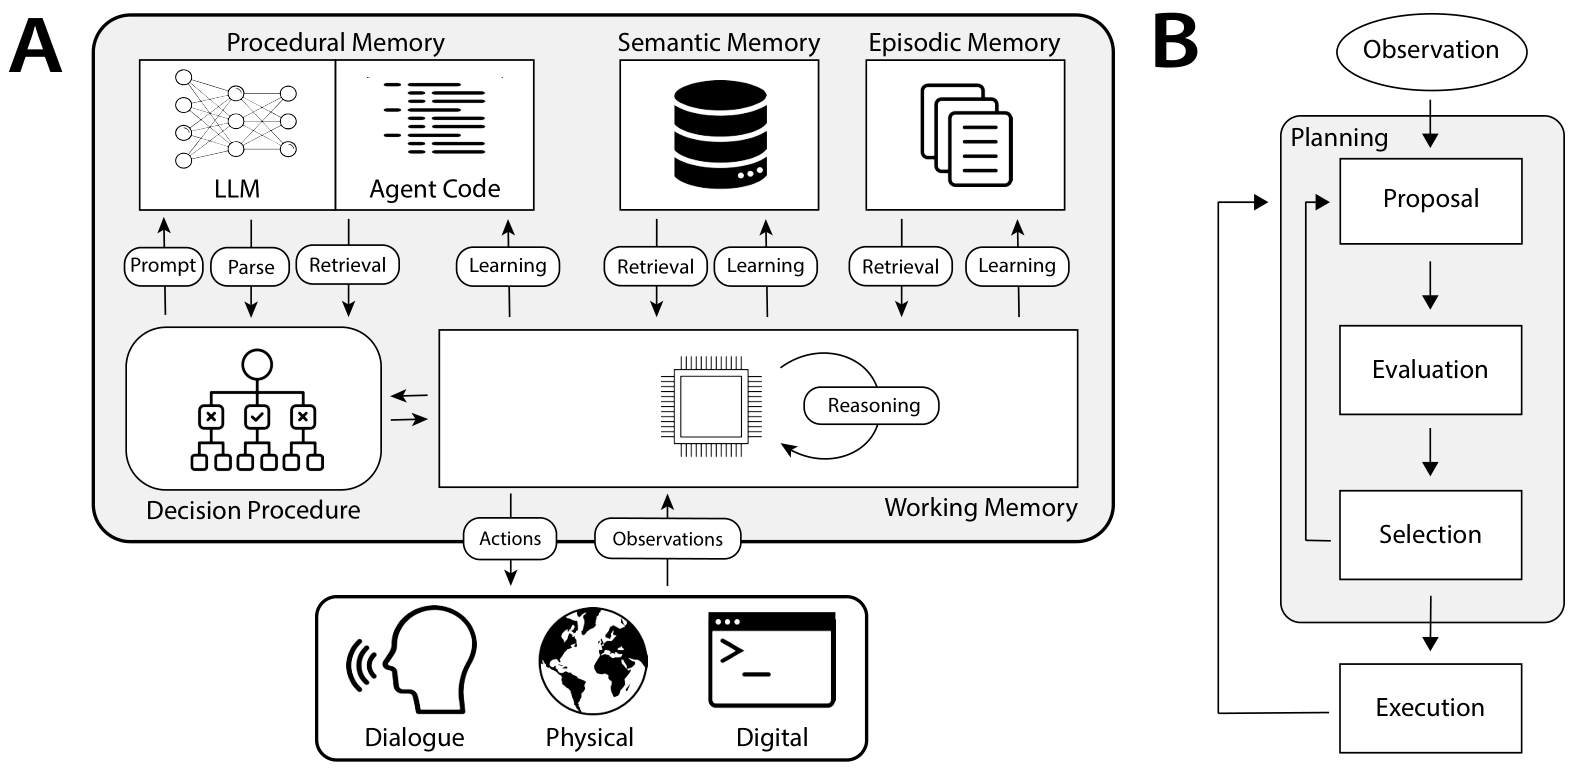
\includegraphics[width=\linewidth,height=0.6\textheight,keepaspectratio]{images/agentic-models-memory/coala_fig4_architecture.png}
        \column{0.38\textwidth}
        \begin{itemize}\itemsep0.4em
            \item \textbf{Working:} the current decision cycle. In practice, the context.
            \item \textbf{Episodic:} what happened.
            \item \textbf{Semantic:} what is true.
            \item \textbf{Procedural:} how to act. \emph{Implicit} in the weights, \emph{explicit} in the agent's code.
        \end{itemize}
    \end{columns}
    \vspace{0.3em}
    \begin{itemize}
        \item Memory is reached by internal actions: \emph{retrieval} reads it, \emph{learning} writes it. \alert{Writing procedural memory is the riskiest}: it can introduce bugs or subvert the designer's intent.
    \end{itemize}
    \src{Sumers, Yao, Narasimhan and Griffiths, ``Cognitive Architectures for Language Agents'' (CoALA), \href{https://arxiv.org/abs/2309.02427}{arXiv:2309.02427}, Figure 4.}
\end{frame}

\begin{frame}{Where Each Memory Type Lives in Real Systems}
    \begin{center}
    \small
    \renewcommand{\arraystretch}{1.2}
    \begin{adjustbox}{max width=\linewidth}\begin{tabular}{>{\raggedright\arraybackslash}p{2.9cm}>{\raggedright\arraybackslash}p{5.2cm}>{\raggedright\arraybackslash}p{5.0cm}}
        \toprule
        \textbf{Type} & \textbf{Research systems} & \textbf{Products} \\
        \midrule
        Working & MemGPT working context & the context window \\
        Episodic & MemGPT recall storage, Generative Agents memory stream & Claude chat search, ChatGPT chat history \\
        Semantic & Mem0 facts, Zep entity graph & Claude topics, ChatGPT saved memories \\
        Procedural, explicit & Voyager skills, Agent Workflow Memory & Agent Skills \\
        Procedural, implicit & fine-tuning and agentic RL & the model weights \\
        \bottomrule
    \end{tabular}\end{adjustbox}
    \end{center}
    \begin{itemize}\itemsep0.4em
        \item \textbf{Episodic memory is the neglected one.} A 2025 position paper calls it the missing piece for long-term agents.
    \end{itemize}
    \src{Mapping is a synthesis of the cited systems, after Sumers et al., \href{https://arxiv.org/abs/2309.02427}{arXiv:2309.02427}. Pink et al., ``Position: Episodic Memory is the Missing Piece,'' \href{https://arxiv.org/abs/2502.06975}{arXiv:2502.06975}.}
\end{frame}

\begin{frame}{Lineage 1: The Agent Manages Its Own Memory (MemGPT)}
    \begin{columns}[T,onlytextwidth]
        \column{0.56\textwidth}
        \begin{itemize}\itemsep0.4em
            \item \textbf{Idea.} Borrow the operating-system memory hierarchy. The LLM pages information in and out with \emph{function calls}.
            \item \textbf{Main context} (the prompt): read-only instructions, a fixed-size \emph{working context} the model can edit, and a FIFO queue of messages.
            \item \textbf{External context:} \emph{recall storage} (every message) and \emph{archival storage} (arbitrary text).
            \item \textbf{Memory pressure.} A warning fires at about 70\% of the window. At 100\% the queue is flushed and summarised.
            \item \textbf{Result.} Deep memory retrieval with GPT-4: 32.1\% without, \textbf{92.5\%} with.
        \end{itemize}
        \column{0.42\textwidth}
        \centering
        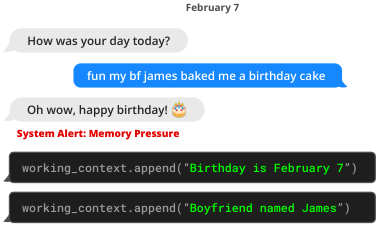
\includegraphics[width=0.9\linewidth,height=0.3\textheight,keepaspectratio]{images/agentic-models-memory/memgpt_fig1_memory_write.png}

        \vspace{0.3em}
        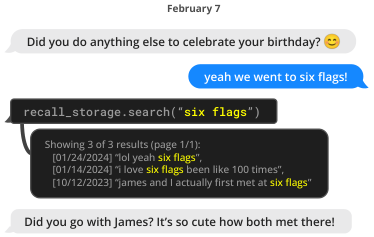
\includegraphics[width=0.9\linewidth,height=0.3\textheight,keepaspectratio]{images/agentic-models-memory/memgpt_fig3_architecture.png}
    \end{columns}
    \vspace{0.2em}
    \src{Packer et al., ``MemGPT: Towards LLMs as Operating Systems,'' \href{https://arxiv.org/abs/2310.08560}{arXiv:2310.08560}, Figures 1 and 3, Table 2. Top: a write after a pressure alert. Bottom: a search of recall storage.}
\end{frame}

\begin{frame}{Lineage 2: A Pipeline Manages Memory (Generative Agents)}
    \begin{columns}[T,onlytextwidth]
        \column{0.5\textwidth}
        \begin{itemize}\itemsep0.4em
            \item \textbf{Memory stream.} A time-stamped log of observations, plans and reflections.
            \item \textbf{Retrieval score}, each term normalised to $[0,1]$:
            \[
                \text{score} = \text{recency} + \text{importance} + \text{relevance}
            \]
            \item Recency decays by 0.995 per game hour. Importance is rated 1 to 10 by the LLM.
            \item \textbf{Reflection.} When summed importance passes 150, the agent writes 5 insights. Episodes become \emph{semantic} memory.
        \end{itemize}
        \column{0.48\textwidth}
        \centering
        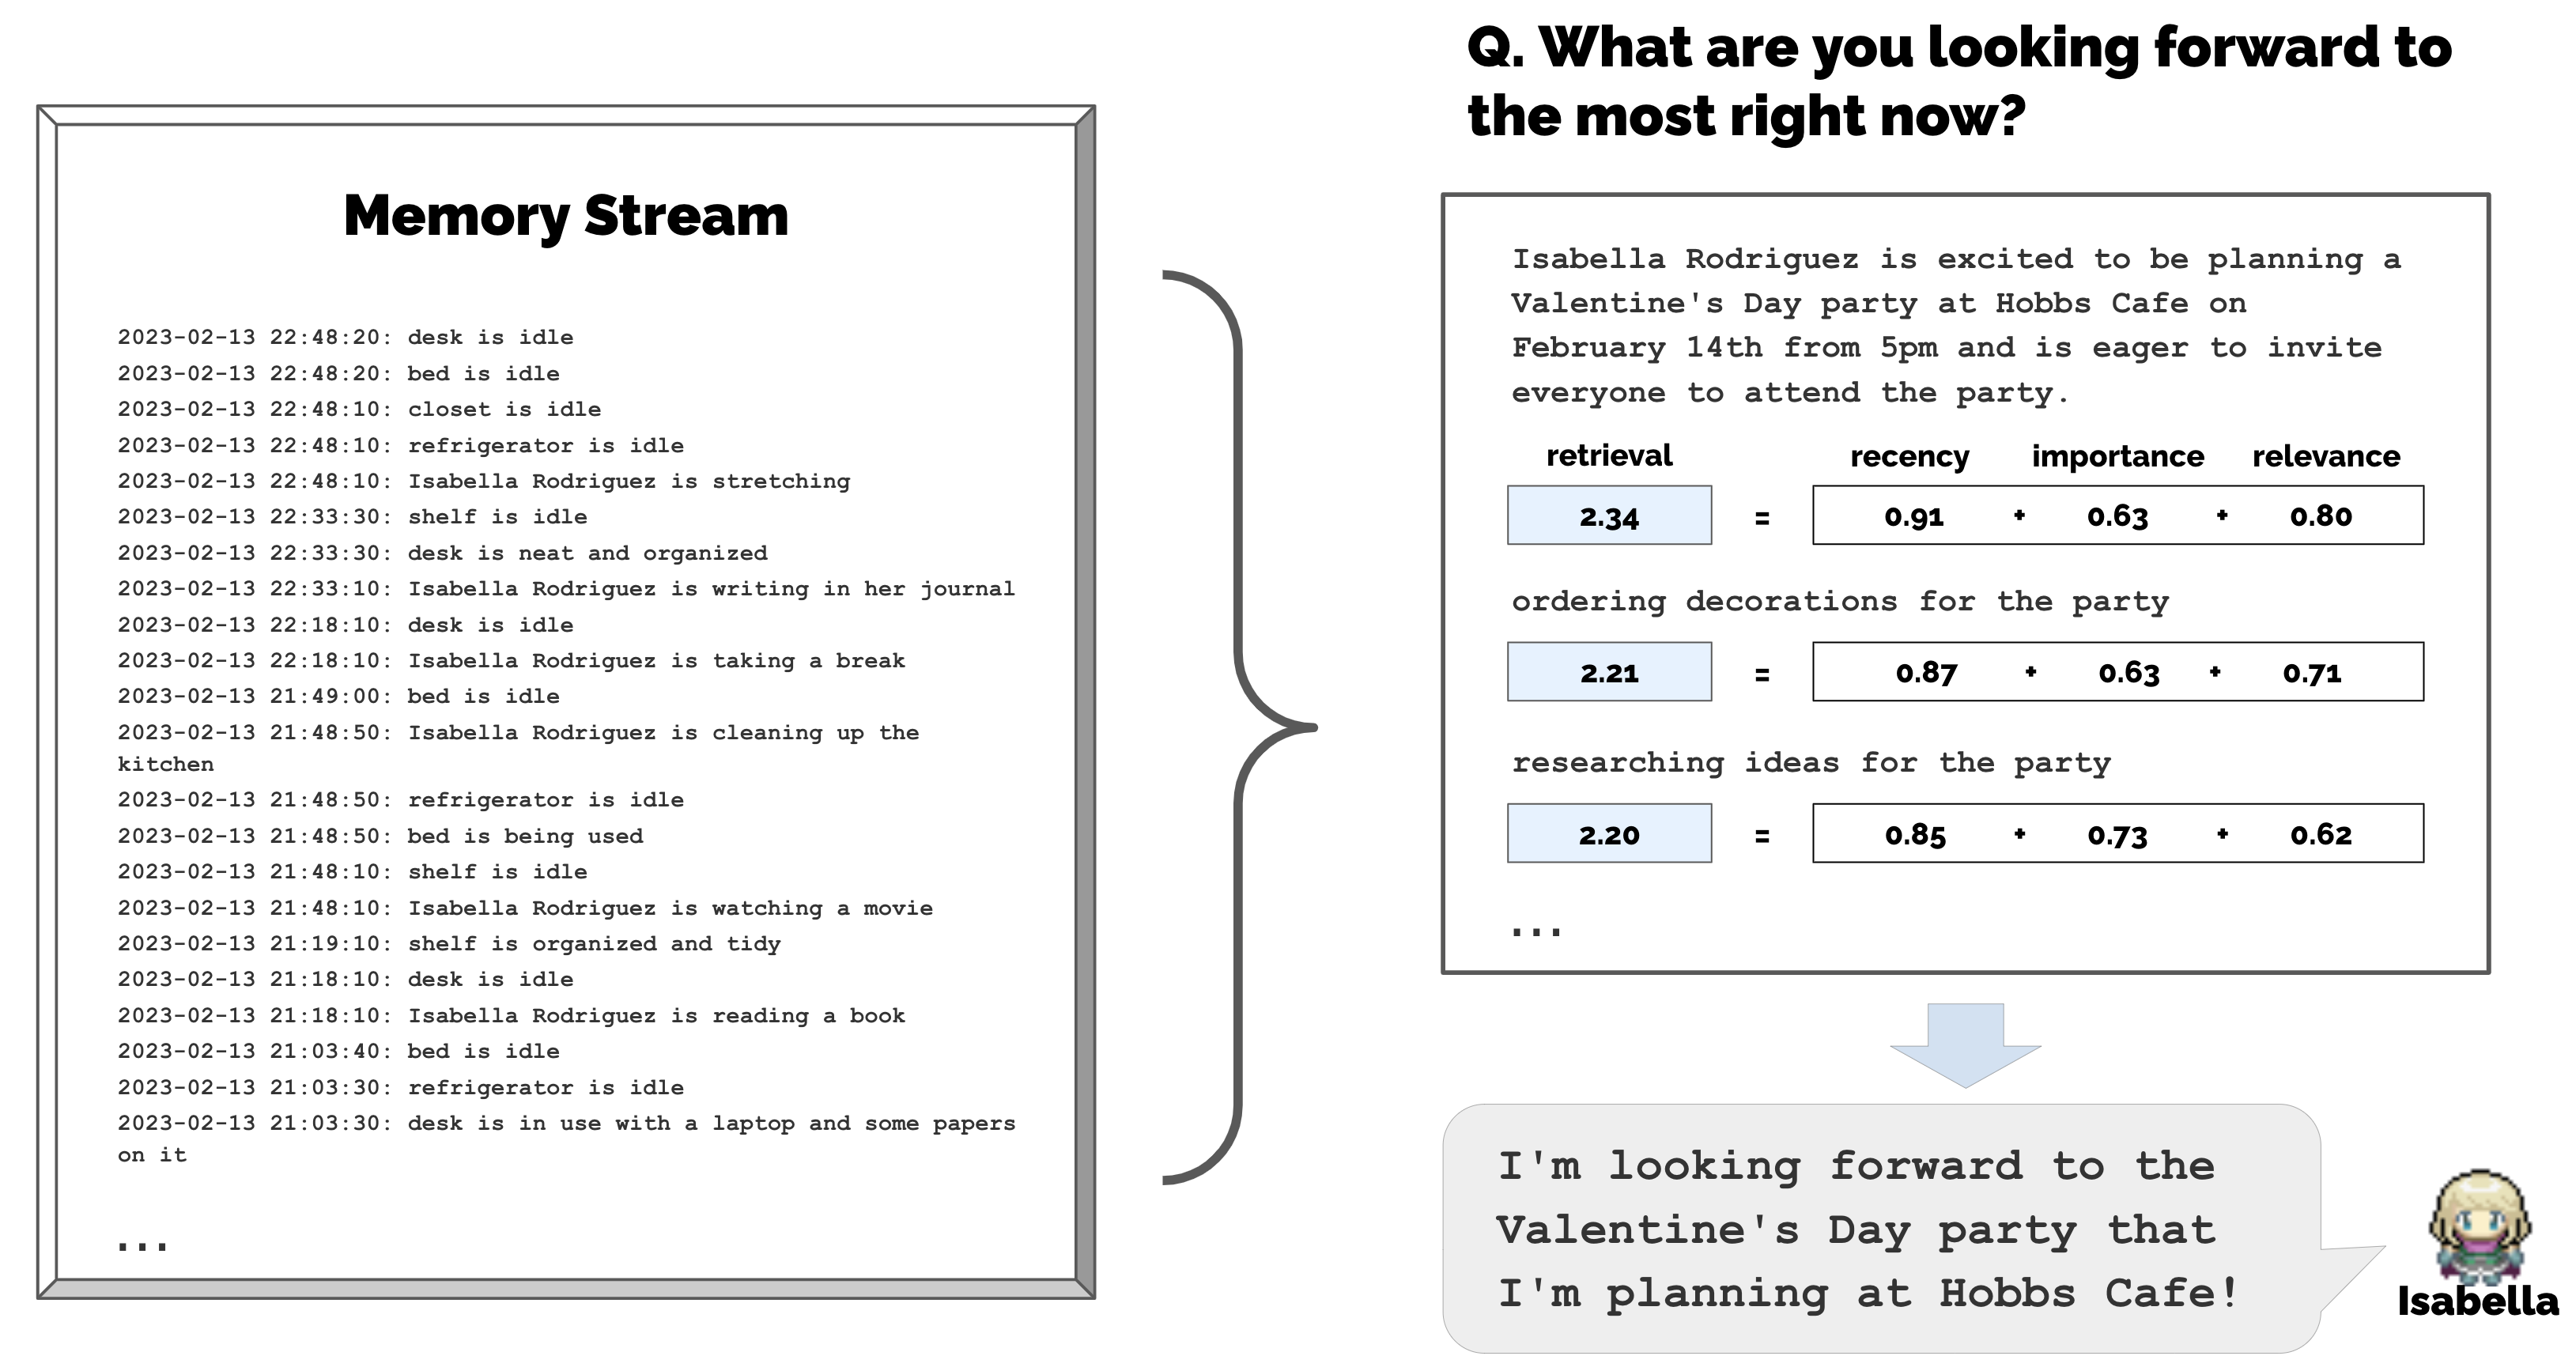
\includegraphics[width=\linewidth,height=0.58\textheight,keepaspectratio]{images/agentic-models-memory/genagents_fig6_retrieval.png}
    \end{columns}
    \vspace{0.2em}
    \takeaway{An origin idea. Systems since 2025 replace the hand-tuned score with \textbf{LLM-decided update operations} and temporal invalidation.}
    \src{Park et al., ``Generative Agents: Interactive Simulacra of Human Behavior,'' \href{https://arxiv.org/abs/2304.03442}{arXiv:2304.03442}, Figure 6.}
\end{frame}

\begin{frame}{The Write Path: Extract, Compare, Mutate}
    \begin{center}
    \small
    \renewcommand{\arraystretch}{1.25}
    \begin{adjustbox}{max width=\linewidth}\begin{tabular}{>{\raggedright\arraybackslash}p{1.9cm}>{\raggedright\arraybackslash}p{4.0cm}>{\raggedright\arraybackslash}p{7.2cm}}
        \toprule
        \textbf{System} & \textbf{Store} & \textbf{What happens on a write} \\
        \midrule
        Mem0 & facts, optionally a graph & LLM extracts facts, then chooses \texttt{ADD}, \texttt{UPDATE}, \texttt{DELETE} or \texttt{NOOP} \\
        A-MEM & linked notes & the LLM links a new note to similar ones, then \emph{evolves} the old notes \\
        Zep & temporal knowledge graph & on a contradiction, the old edge is \emph{invalidated}, not deleted \\
        \bottomrule
    \end{tabular}\end{adjustbox}
    \end{center}
    \begin{itemize}\itemsep0.45em
        \item \textbf{What changed.} ``Append and embed'' became an LLM-in-the-loop write. Cost moves from read time to write time.
        \item \textbf{Asynchronous consolidation.} Letta's sleep-time agent rewrites memory between user turns: about 5$\times$ less test-time compute for the same accuracy.
    \end{itemize}
    \src{Chhikara et al., \href{https://arxiv.org/abs/2504.19413}{arXiv:2504.19413}. Xu et al., ``A-Mem,'' \href{https://arxiv.org/abs/2502.12110}{arXiv:2502.12110}. Rasmussen et al., ``Zep,'' \href{https://arxiv.org/abs/2501.13956}{arXiv:2501.13956}. Lin et al., ``Sleep-time Compute,'' \href{https://arxiv.org/abs/2504.13171}{arXiv:2504.13171}.}
\end{frame}

\begin{frame}{Learning the Write Policy with Reinforcement Learning}
    \centering
    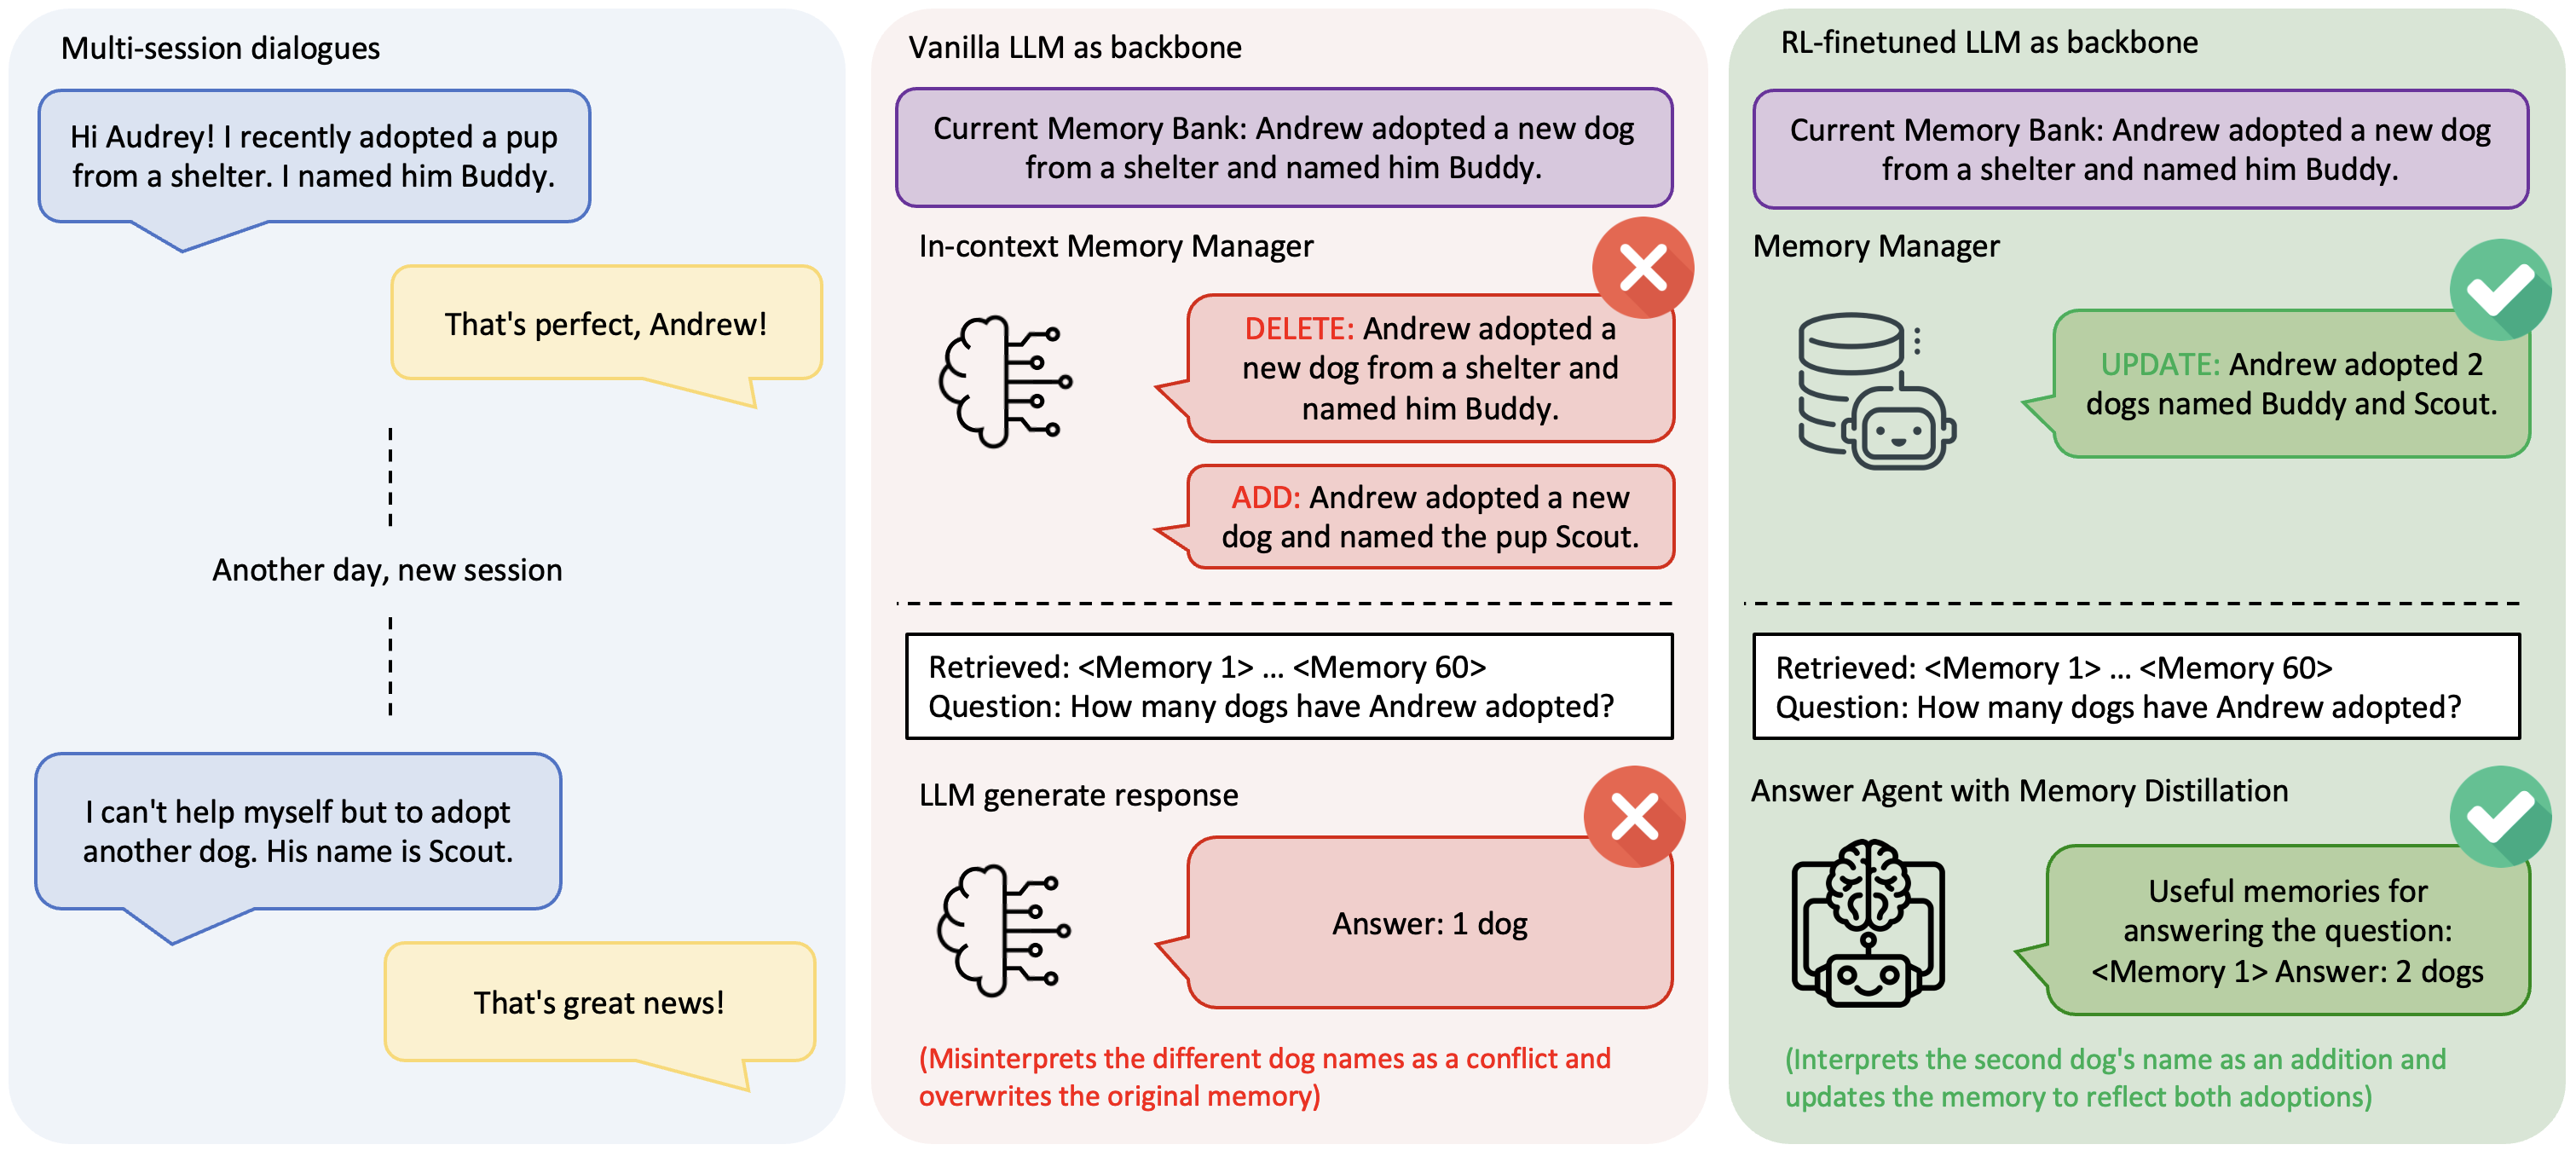
\includegraphics[width=0.95\linewidth,height=0.5\textheight,keepaspectratio]{images/agentic-models-memory/memoryr1_fig1_usecase.png}
    \begin{center}
    \small
    \renewcommand{\arraystretch}{1.15}
    \begin{adjustbox}{max width=\linewidth}\begin{tabular}{lll}
        \toprule
        \textbf{Method} & \textbf{What the policy controls} & \textbf{Headline, from a final-answer reward only} \\
        \midrule
        Memory-R1 (figure) & discrete operations on a store & +48\% F1 over Mem0, 152 training pairs \\
        MEM1 & a state that \emph{replaces} the context & 3.5$\times$ performance, 3.7$\times$ less memory \\
        MemAgent & a 1,024-token overwrite buffer & trained at 8K, 71\% at 3.5M tokens \\
        \bottomrule
    \end{tabular}\end{adjustbox}
    \end{center}
    \src{Figure: Yan et al., ``Memory-R1,'' \href{https://arxiv.org/abs/2508.19828}{arXiv:2508.19828}, Figure 1. Zhou et al., ``MEM1,'' \href{https://arxiv.org/abs/2506.15841}{arXiv:2506.15841}. Yu et al., ``MemAgent,'' \href{https://arxiv.org/abs/2507.02259}{arXiv:2507.02259}. Some numbers were extracted by a summarising tool.}
\end{frame}

\begin{frame}{Industry Converged on Something Simpler: Files, Tools, a Policy}
    \begin{columns}[T,onlytextwidth]
        \column{0.6\textwidth}
        \begin{itemize}\itemsep0.45em
            \item \textbf{The file system as memory.} Manus recites a \texttt{todo.md} across about 50 tool calls per task. Compression is \emph{restorable}: keep the URL, drop the page.
            \item \textbf{A memory tool.} Claude's API exposes a \texttt{/memories} directory. The injected protocol: view memory first, assume interruption.
            \item \textbf{The surprise.} An agent with plain \texttt{grep} and file tools scored 74.0\% on LoCoMo, above a dedicated graph memory at 68.5\%.
        \end{itemize}
        \column{0.37\textwidth}
        \centering
        \begin{adjustbox}{max width=\linewidth}\begin{tikzpicture}[font=\footnotesize, >=Stealth,
            b/.style={draw, rounded corners=2pt, minimum width=3.6cm, minimum height=0.7cm, align=center}]
            \node[b, fill=darkorange!20] (p) at (0,3.2) {\textbf{Policy}: what to write, when};
            \node[b, fill=KAUSTcyan!20] (t) at (0,2.0) {\textbf{Tools}: view, write, search};
            \node[b, fill=gray!12] (f) at (0,0.8) {\textbf{Files}: notes, progress, todo};
            \node[b, dashed, text=gray] (v) at (0,-0.4) {optional vector or graph store};
            \draw[->, thick] (p) -- (t);
            \draw[->, thick] (t) -- (f);
            \draw[->, thick, gray] (f) -- (v);
        \end{tikzpicture}\end{adjustbox}
    \end{columns}
    \vspace{0.3em}
    \takeaway{A 2026 study of 12 systems on 5 workloads: \textbf{no single architecture dominates}.}
    \src{Ji, ``Context Engineering for AI Agents: Lessons from Building Manus'' (2025). Anthropic, memory tool docs. Letta, ``Benchmarking AI Agent Memory'' (2025, vendor). Zhou et al., ``Are We Ready For An Agent-Native Memory System?'' \href{https://arxiv.org/abs/2606.24775}{arXiv:2606.24775}.}
\end{frame}

\begin{frame}{Procedural Memory: Skills the Agent Can Reuse}
    \centering
    \begin{adjustbox}{max width=\linewidth}\begin{tikzpicture}[font=\footnotesize, >=Stealth,
        b/.style={draw, rounded corners=2pt, minimum width=3.9cm, minimum height=1.25cm, align=center, text width=3.7cm}]
        \node[b, fill=gray!12] (a) at (0,0) {\textbf{Voyager (2023)}\\executable code skills, retrieved by embedding};
        \node[b, fill=KAUSTcyan!18] (b) at (4.6,0) {\textbf{Workflow Memory (2024)}\\workflows induced from past trajectories};
        \node[b, fill=darkorange!20] (c) at (9.2,0) {\textbf{Agent Skills (2025)}\\a folder: instructions, scripts, resources};
        \draw[->, thick] (a) -- (b);
        \draw[->, thick] (b) -- (c);
    \end{tikzpicture}\end{adjustbox}
    \vspace{0.6em}
    \begin{itemize}\itemsep0.45em
        \item \textbf{Voyager.} A growing skill library gave 3.3$\times$ more unique items and 15.3$\times$ faster tech-tree milestones in Minecraft.
        \item \textbf{Agent Workflow Memory.} Relative success up 24.6\% on Mind2Web and 51.1\% on WebArena.
        \item \textbf{Agent Skills} use \emph{progressive disclosure}: only a name and description sit in the prompt. Instructions and scripts load on demand, like deferred tools.
        \item \alert{A skill from an untrusted source can carry malicious instructions.}
    \end{itemize}
    \src{Wang et al., ``Voyager,'' \href{https://arxiv.org/abs/2305.16291}{arXiv:2305.16291}. Wang, Mao, Fried and Neubig, ``Agent Workflow Memory,'' \href{https://arxiv.org/abs/2409.07429}{arXiv:2409.07429}. Anthropic, ``Equipping agents for the real world with Agent Skills'' (Oct 2025).}
\end{frame}

\begin{frame}{Retrieval-Memory Hybrids: Give the Index a Structure}
    \begin{center}
    \small
    \renewcommand{\arraystretch}{1.2}
    \begin{adjustbox}{max width=\linewidth}\begin{tabular}{>{\raggedright\arraybackslash}p{1.9cm}>{\raggedright\arraybackslash}p{4.9cm}>{\raggedright\arraybackslash}p{2.9cm}>{\raggedright\arraybackslash}p{3.3cm}}
        \toprule
        \textbf{System} & \textbf{Structure built at index time} & \textbf{Memory role} & \textbf{Headline} \\
        \midrule
        RAPTOR & tree of recursive cluster summaries & consolidation & +20\% absolute on QuALITY \\
        MemoRAG & a small model's compressed global memory drafts retrieval clues & global memory & 40.2 against 35.0 for full context \\
        \bottomrule
    \end{tabular}\end{adjustbox}
    \end{center}
    \begin{itemize}
        \item Graph indexes play the same two roles: GraphRAG's community summaries are \textbf{consolidation}, HippoRAG's knowledge graph is \textbf{association}.
    \end{itemize}
    \takeaway{Flat RAG only recognises chunks. Each of these \textbf{precomputes a kind of memory} for sense-making or association.}
    \src{Sarthi et al., \href{https://arxiv.org/abs/2401.18059}{arXiv:2401.18059}. Edge et al., \href{https://arxiv.org/abs/2404.16130}{arXiv:2404.16130}. Jim\'enez Guti\'errez et al., \href{https://arxiv.org/abs/2405.14831}{arXiv:2405.14831}. Qian et al., \href{https://arxiv.org/abs/2409.05591}{arXiv:2409.05591}. Su, Berkeley CS294 (2025).}
\end{frame}

\begin{frame}{Structure Has a Price}
    \begin{columns}[T,onlytextwidth]
        \column{0.55\textwidth}
        \begin{itemize}\itemsep0.45em
            \item \textbf{Simple facts get worse.} GraphRAG, LightRAG and RAPTOR drop on plain factual questions against a strong dense retriever.
            \item \textbf{Graph indexes are expensive.} A GraphRAG answer reads about 610,000 tokens of community reports. LightRAG needs under 100.
        \end{itemize}
        \column{0.42\textwidth}
        \centering
        \small
        \renewcommand{\arraystretch}{1.2}
        \begin{adjustbox}{max width=\linewidth}\begin{tabular}{lcc}
            \toprule
            \textbf{MemoryAgentBench} & \textbf{Retrieval} & \textbf{Overall} \\
            \midrule
            BM25 & 60.5 & \\
            GraphRAG & 40.9 & 19.9 \\
            MIRIX & 47.5 & 34.3 \\
            \bottomrule
        \end{tabular}\end{adjustbox}

        \vspace{0.5em}
        {\footnotesize MIRIX self-reports 85.4\% on LoCoMo.}
    \end{columns}
    \vspace{0.3em}
    \caveat{\textbf{Not all memory should be external.} On deep compositions of facts, models using retrieval ``fail badly''. A grokked transformer is near perfect.}
    \src{Jim\'enez Guti\'errez et al., ``HippoRAG 2,'' \href{https://arxiv.org/abs/2502.14802}{arXiv:2502.14802}. Guo et al., ``LightRAG,'' \href{https://arxiv.org/abs/2410.05779}{arXiv:2410.05779}. Hu et al., \href{https://arxiv.org/abs/2507.05257}{arXiv:2507.05257}. Su, Berkeley CS294 (2025).}
\end{frame}

\begin{frame}{The LoCoMo Dispute: Read Memory Benchmarks Carefully}
    \begin{columns}[T,onlytextwidth]
        \column{0.52\textwidth}
        \centering
        \begin{adjustbox}{max width=\linewidth}\begin{tikzpicture}
            \begin{axis}[
                xbar, bar width=8pt, width=6.3cm, height=5.4cm,
                xmin=60, xmax=79, xtick={60,65,70,75}, xlabel={LoCoMo judge score (\%)},
                symbolic y coords={Zep in Mem0 paper,Mem0,Mem0 graph,Full context,Letta files,Zep own rerun},
                ytick=data, y tick label style={font=\scriptsize},
                x label style={font=\scriptsize}, x tick label style={font=\scriptsize},
                nodes near coords, nodes near coords style={font=\tiny},
                axis lines*=left, xmajorgrids, grid style={gray!20}, enlarge y limits=0.12]
                \addplot[fill=KAUSTcyan!55, draw=KAUSTcyan!70!black] coordinates {(65.99,Zep in Mem0 paper) (66.88,Mem0) (68.44,Mem0 graph) (72.90,Full context) (74.0,Letta files) (75.14,Zep own rerun)};
            \end{axis}
        \end{tikzpicture}\end{adjustbox}
        \column{0.46\textwidth}
        \begin{itemize}\itemsep0.45em
            \item In Mem0's own paper, \alert{full context beats every memory layer}.
            \item LoCoMo conversations are only 16K to 26K tokens. They fit in context, and they contain no knowledge-update tests.
            \item \textbf{Defensible claim:} memory layers trade about 4 to 7 points for roughly 10$\times$ lower latency and far fewer tokens.
        \end{itemize}
    \end{columns}
    \vspace{0.2em}
    \caveat{Every number here is \textbf{vendor-reported}. There is no independent replication. Prefer LongMemEval and MemoryAgentBench.}
    \src{Chhikara et al., \href{https://arxiv.org/abs/2504.19413}{arXiv:2504.19413}, Table 2. Chalef and Rasmussen, ``Is Mem0 Really SOTA in Agent Memory?'' (Zep blog, 2025). Letta, ``Benchmarking AI Agent Memory'' (2025). Maharana et al., ``LoCoMo,'' \href{https://arxiv.org/abs/2402.17753}{arXiv:2402.17753}.}
\end{frame}

\begin{frame}{Memory in Products, and What Nobody Has Solved}
    \begin{center}
    \small
    \renewcommand{\arraystretch}{1.2}
    \begin{adjustbox}{max width=\linewidth}\begin{tabular}{>{\raggedright\arraybackslash}p{1.6cm}>{\raggedright\arraybackslash}p{5.0cm}>{\raggedright\arraybackslash}p{6.4cm}}
        \toprule
        \textbf{Product} & \textbf{Two mechanisms} & \textbf{User controls} \\
        \midrule
        Claude & topics saved during chats, plus chat search as a tool & editable topics, incognito chats, sensitive categories excluded by default \\
        ChatGPT & saved memories, plus reference to chat history & temporary chats, memory sources shown, auto-updating since June 2026 \\
        Gemini & personal context from past chats & on by default, Temporary Chats \\
        \bottomrule
    \end{tabular}\end{adjustbox}
    \end{center}
    \begin{itemize}\itemsep0.4em
        \item \textbf{Forgetting is the weakest skill.} Multi-hop conflict resolution peaks at about 28\% for every method in MemoryAgentBench.
        \item \textbf{Governance gap.} A 2026 survey of 435 works finds research focused on accumulating state, not on \alert{governing, recovering or relinquishing} it.
    \end{itemize}
    \src{Anthropic Help Center, chat search and memory (2026). OpenAI, Memory FAQ and 2026 release notes. Google, Gemini Temporary Chats (2025). Hu et al., \href{https://arxiv.org/abs/2507.05257}{arXiv:2507.05257}. Ding et al., ``Always-On Agents,'' \href{https://arxiv.org/abs/2606.30306}{arXiv:2606.30306}.}
\end{frame}

\begin{frame}{Memory: What to Remember}
    \begin{itemize}\itemsep0.4em
        \item A long context is not a memory. Models lose 30 to 60\% on long histories, and context has a cost.
        \item \textbf{Three types} to design for: episodic (what happened), semantic (what is true), procedural (how to act).
        \item Systems differ most in their \textbf{write policy}: hand-tuned scores, LLM-chosen operations, or a policy learned with RL.
        \item Structured retrieval adds sense-making and association, and pays in indexing cost and simple-fact accuracy.
        \item In practice, memory is \textbf{files, tools and a policy}. Benchmarks in this area are vendor-run and disputed.
    \end{itemize}
    \vspace{0.4em}
    \takeaway{\textbf{Next.} A sub-agent with its own context window is also a memory strategy. When is splitting the work across agents worth it?}
\end{frame}
